\documentclass{article}
\usepackage{graphicx} % Required for inserting images
\usepackage{xcolor}
\usepackage{listings}
\usepackage{float} 
\usepackage[justification=centering]{caption}
\definecolor{mGreen}{rgb}{0,0.6,0}
\definecolor{mGray}{rgb}{0.5,0.5,0.5}
\definecolor{mPurple}{rgb}{0.58,0,0.82}
\definecolor{backgroundColour}{rgb}{0.95,0.95,0.92}
\lstdefinestyle{PythonStyle}{
    backgroundcolor=\color{backgroundColour},   
    commentstyle=\color{mGreen},
    keywordstyle=\color{magenta},
    numberstyle=\tiny\color{mGray},
    stringstyle=\color{mPurple},
    basicstyle=\footnotesize,
    breakatwhitespace=false,         
    breaklines=true,                 
    captionpos=b,                    
    keepspaces=true,                 
    numbers=left,                    
    numbersep=5pt,                  
    showspaces=false,                
    showstringspaces=false,
    showtabs=false,                  
    tabsize=2,
    language=Python
}

\title{Assignment 1: Adaline and Logistic Regression}
\author{Jackie Javier, Pranitha Achanta\\
        The University of New Mexico\\
        CS429}
\date{Due 2/13/2026}

\begin{document}

\maketitle

\section{Task 1}
The bias is transformed into an extra weight by adding an additional 1 value to each sample in the training dataset. The weight that will then be multiplied by this 1 value is exactly equivalent to the original bias, as bias updates are the same as weight updates (for Adaline and Logistic Regression), except for the multiplication by the sample. Since the multiplication for the bias will specifically be by a factor of 1, the bias remains unaffected by the sample despite being absorbed by the weight vector. \\
The line of code that adds a column of ones to the 2D sample array is as follows:
\begin{lstlisting}[style=PythonStyle]
X_bias = np.hstack([X, np.ones((X.shape[0], 1))])
\end{lstlisting}
With this update, all references to b\_ can be removed. The net\_input also remains equivalent, as the bias addition will still occur as $+ (b\_ * 1)$.

\section{Task 2}
Done, just writeup! epochs = 60 and learning rate = 0.01

\begin{figure}[H]
    \centering
    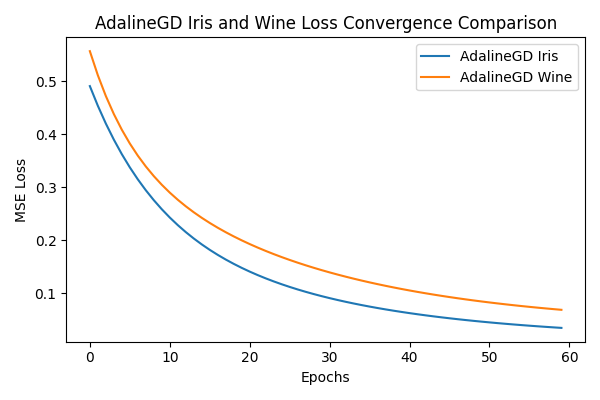
\includegraphics[width=1.0\linewidth]{task2_ada.png}
    \caption{}
    \label{fig:placeholder}
\end{figure}

here

\begin{figure}[H]
    \centering
    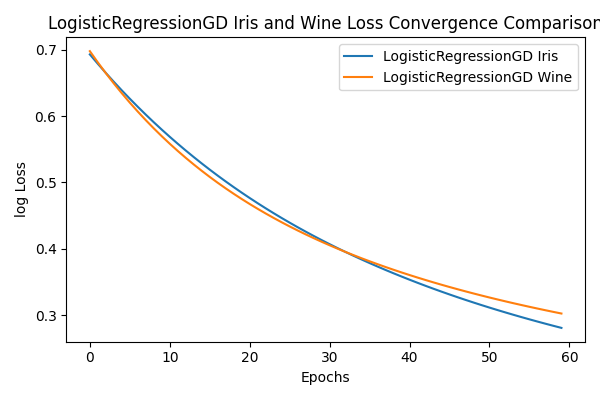
\includegraphics[width=1.0\linewidth]{task2_lr.png}
    \caption{}
    \label{fig:placeholder}
\end{figure}

here

\section{Task 3}
Done, just writeup! epochs = 500 and learning rate = 0.001

\begin{figure}[H]
    \centering
    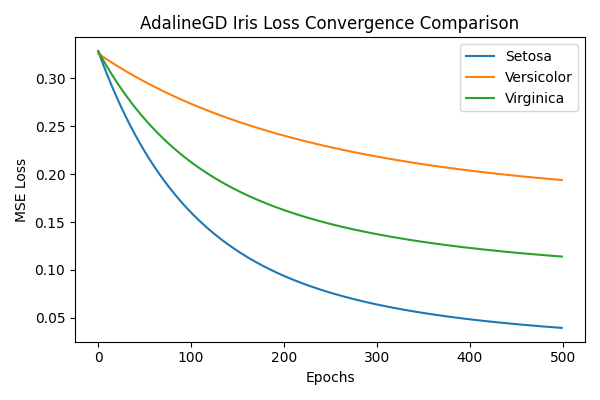
\includegraphics[width=1.0\linewidth]{task3_compare.png}
    \caption{}
    \label{fig:placeholder}
\end{figure}

here

\section{Task 4}
Done? epochs = 60 and learning rate = 0.01

\begin{figure}[H]
    \centering
    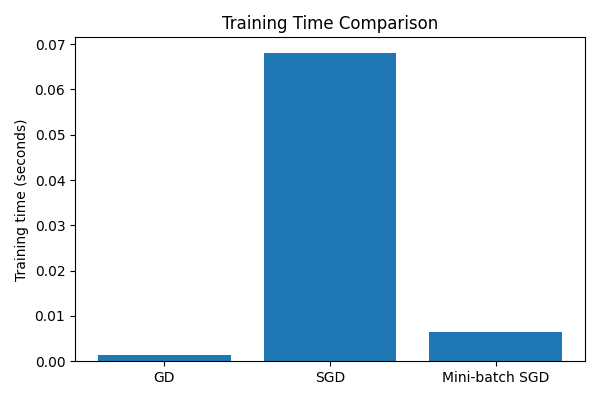
\includegraphics[width=1.0\linewidth]{task4_time.png}
    \caption{}
    \label{fig:placeholder}
\end{figure}

here

\begin{figure}[H]
    \centering
    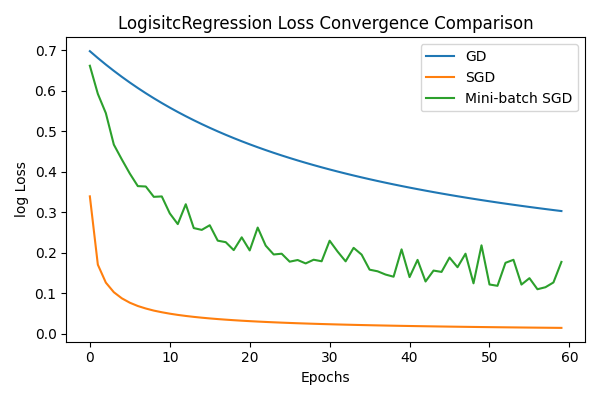
\includegraphics[width=1.0\linewidth]{task4_compare.png}
    \caption{}
    \label{fig:placeholder}
\end{figure}

here

\end{document}
